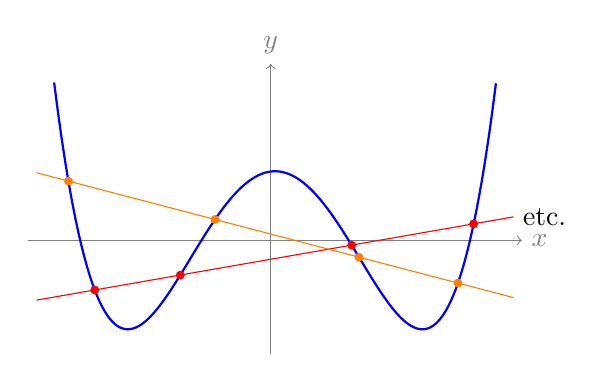
\begin{tikzpicture}[x=1.1cm,y=1.6cm,line cap=round,line join=round]
  % schematic quartic-type curve and two lines, each meeting it in four points
  \draw[->,gray] (-2.8,0) -- (2.9,0) node[right] {$x$};
  \draw[->,gray] (0,-0.9) -- (0,1.4) node[above] {$y$};
  \draw[thick,blue,domain=-2.5:2.6,samples=120,smooth]
    plot (\x,{0.15*(\x+2.2)*(\x+0.8)*(\x-0.9)*(\x-2.3)});
  \draw[red] (-2.7,{0.12*(-2.7)-0.15}) -- (2.8,{0.12*2.8-0.15});
  \draw[orange] (-2.7,{-0.18*(-2.7)+0.05}) -- (2.8,{-0.18*2.8+0.05});
  \foreach \p in {-2.032,-1.044,0.934,2.342}
    \fill[red] (\p,{0.12*\p-0.15}) circle (1.6pt);
  \foreach \p in {-2.336,-0.644,1.018,2.161}
    \fill[orange] (\p,{-0.18*\p+0.05}) circle (1.6pt);
  \node[right] at (2.8,{0.12*2.8-0.15}) {etc.};
\end{tikzpicture}
